\subsection{Wellendiskussion}
\label{sec:wellen:diskussionwellenform}
W"ahrend wir anschliessend mit der Rekursionsformel L"osungen unserer 
Differentialgleichung geplottet haben, entdeckten wir, dass die Welle ihre Form 
bei den jeweiligen Nullstellen des Profils $p(x)$ wechselt. Vergleichen wir die 
Wellenformen der Abbildungen \ref{fig:wellen:variablec} und 
\ref{fig:wellen:variablea} mit den Abbildungen \ref{fig:wellen:sin-cos} und 
\ref{fig:wellen:sinh-cosh}, stellt sich heraus, dass die L"osung der 
Titelgleichung eng mit der gefundenen L"osung der Gleichung 
(\ref{eq:wellen:lineareDGL}) verwandt ist. So k"onnen die L"osungen des 
Parabelprofils als verschiedene $c$ Werte der linearen Differentialgleichung 
verstanden werden, welche dann in die L"osungsgleichung 
(\ref{eq:wellen:loesunglinearedgl}) eingesetzt werden k"onnen. 
Da aber mit einem $c$ respektive mit einer L"osung der Parabel nur ein Punkt 
und nicht die ganze Funktion beschrieben wird, lassen sich die Konstanten $C_1$ 
und $C_2$ aus der Gleichung \ref{eq:wellen:loesunglinearedgl} nicht mehr 
allgemein bestimmen. Es gibt ausserdem keine reinen trigonometrischen Formen 
mehr, sondern f"ur negative Profill"osungen eine Kombination aus den 
hyperbolischen Funktionen Sinus Hyperbolicus und Cosinus Hyperbolicus und f"ur 
positive eine Kombination aus Sinus und Cosinus.

Die Wellenform sind bei variablem $c$ (Abbildung \ref{fig:wellen:variablec}) 
und $a$ (Abbildung \ref{fig:wellen:variablea}) alle "ahnlich, da sich nichts 
weiteres ver"andert als der Ort der Nullstelle der Parabel. Es "andert sich die 
Wellenl"ange, vor allem wenn die Parabel weiter ge"offnet wird. Die Amplitude 
hingegen wird haupts"achlich vom $c$-Wert beeinflusst. Weiter ist erkennbar, 
dass die Parabelform die Geschwindigkeit der Welle beeinflusst, was zu Beginn 
des Kapitels erw"ahnt wurde, und somit als best"atigt gilt.

\begin{figure}
	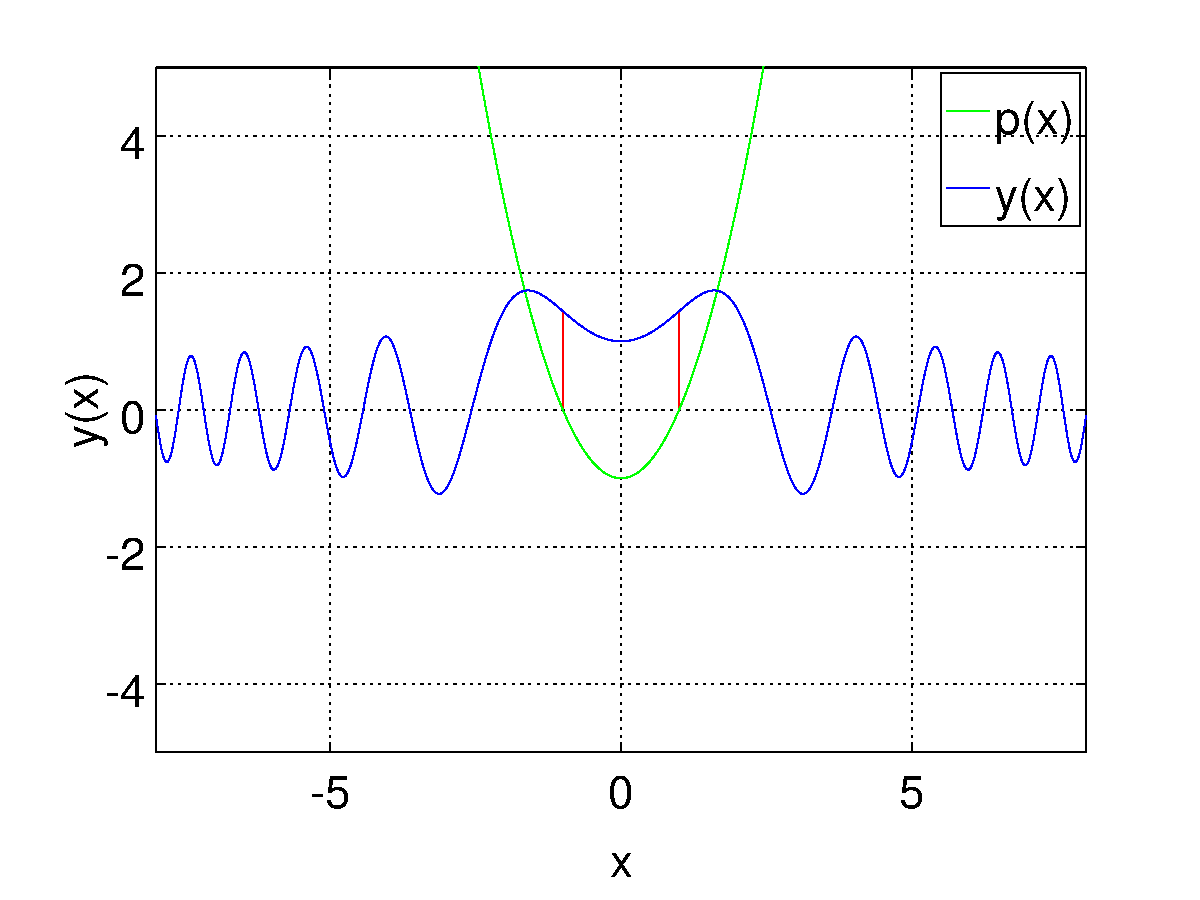
\includegraphics[width=0.51\hsize]{./wellen/images/varc/varc1.pdf}
	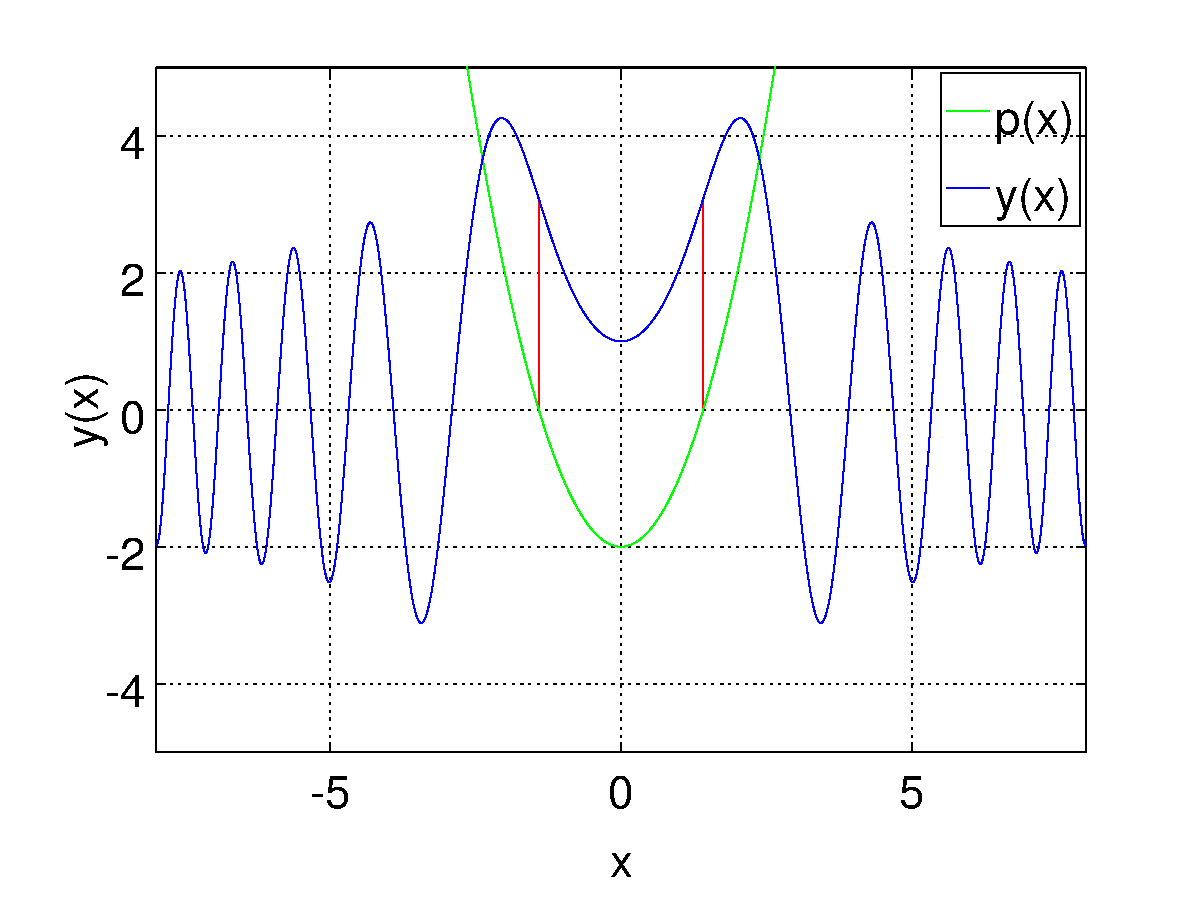
\includegraphics[width=0.51\hsize]{./wellen/images/varc/varc2.pdf}
	\caption{Wellenform mit unterschiedlichen $c$ Werten}
	\label{fig:wellen:variablec}
\end{figure}

\begin{figure}
	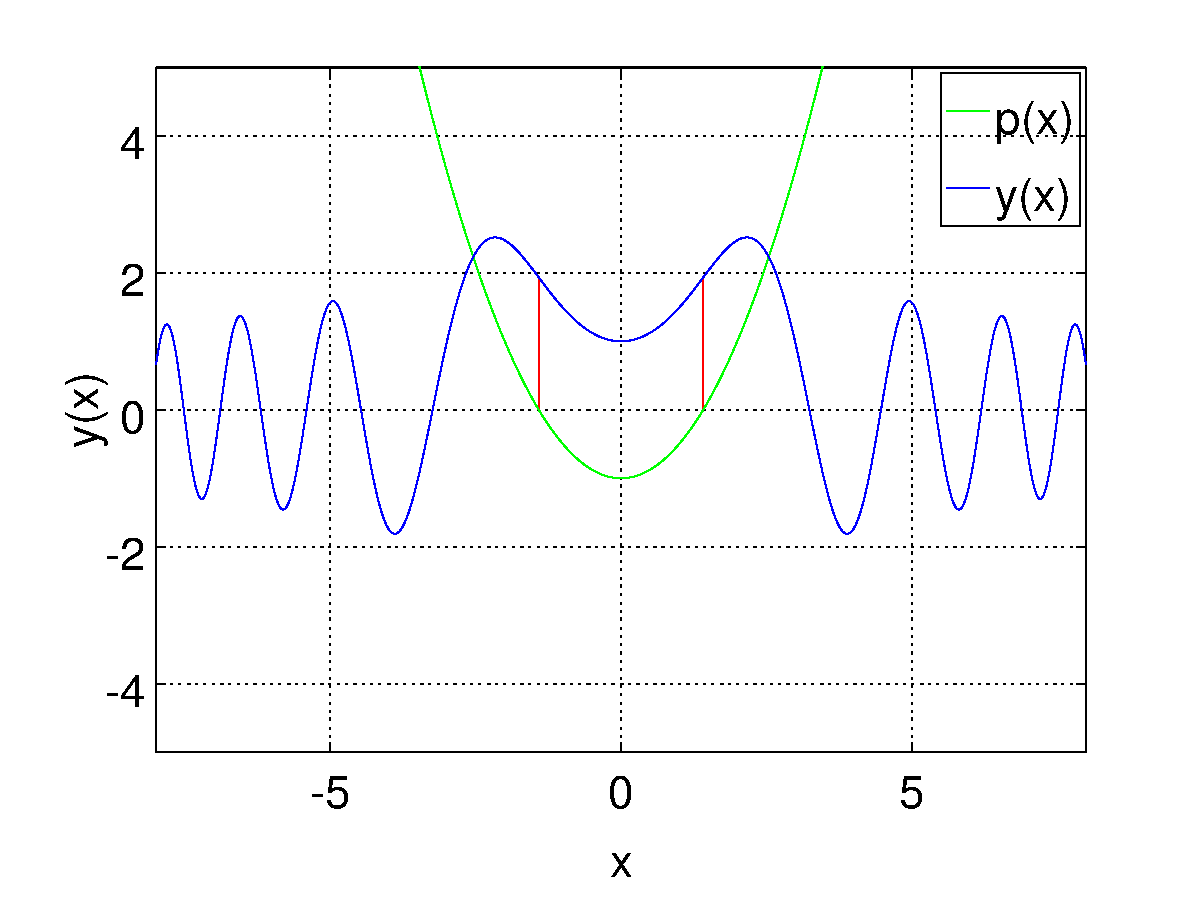
\includegraphics[width=0.51\hsize]{./wellen/images/vara/vara1.pdf}
	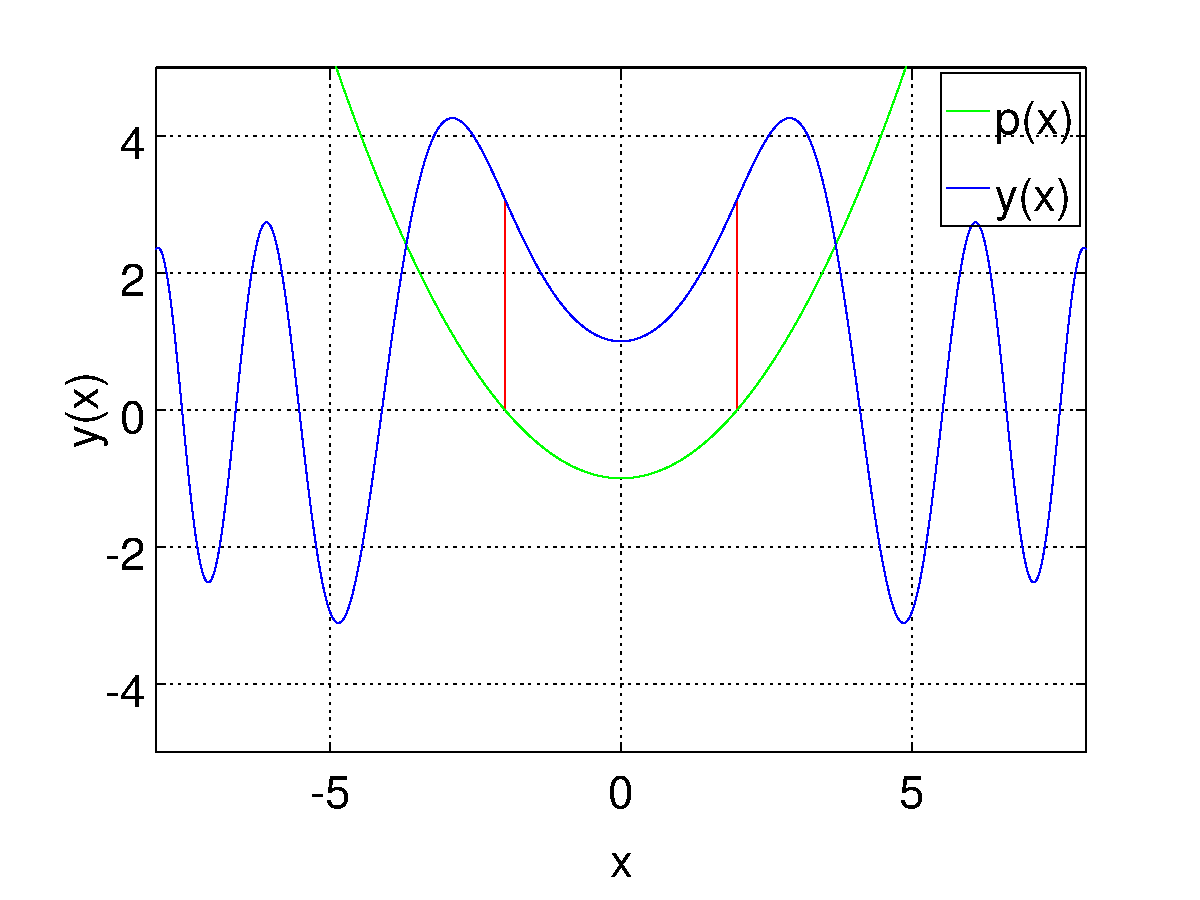
\includegraphics[width=0.51\hsize]{./wellen/images/vara/vara2.pdf}
	\caption{Wellenform bei unterschiedlichen $a$ Werten}
	\label{fig:wellen:variablea}
\end{figure}

Mit dieser Diskussion verlassen wir das parabolische Profil und betrachten 
allgemeinere Aspekte wie Stolpersteine bei der Ausf"uhrung solcher Berechnungen 
oder, wie versprochen, die verallgemeinerte L"osung von Differentialgleichungen 
dieser Art mit einem Profil der Form
\begin{equation*}
p(x) = \sum_{i=0}^{n} \lambda_i x^i.
\end{equation*}
